\chapter{硬件模块介绍}
\section{Chisel3集成的工具}
Chisel3在进行硬件电路描述的同时也提供了一些常用的工具。参考表\ref{chisel-tool}。
\begin{table}[h] %开始一个表格environment,表格的位置是h,here。  
    \centering
    \caption{Chisel3提供的部分小工具} %显示表格的标题  
    \begin{tabular}{l|l} %设置了每一列的宽度,强制转换。  
    \hline  
    \hline  
    名称 & 描述 \\ %用&来分隔单元格的内容 \\表示进入下一行  
    \hline %画一个横线,下面的就都是一样了,这里一共有4行内容  
    Decoupled() & 用于将数据拓展成标准的ready-valid接口 \\  
    \hline %画一个横线,下面的就都是一样了,这里一共有4行内容  
    Flipped() & 用于接口的翻转,Input翻转为Output,Output翻转为Input \\  
    \hline  
    Queue & 输入为Flipped(Decoupled)输出为Decoupled接口类型的FIFO \\  
    \hline  
    MEM & 同步写、异步读的RAM \\  
    \hline  
    \hline  
    \end{tabular}  
    \label{chisel-tool}
\end{table}  
\begin{figure}[h]
    \centering
    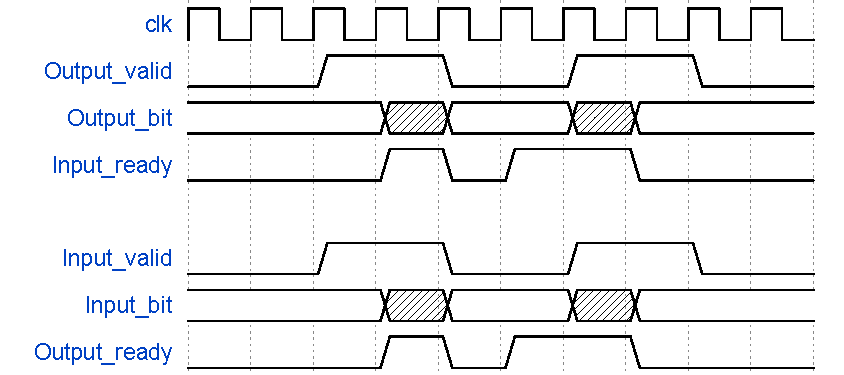
\includegraphics{../pdf/decoupled.pdf}\\
    \caption{Decoupled与Flipped(Decoupled)接口波形图}
    \label{decoupled_w}
\end{figure}

本文大量使用了\emph{Decoupled}类型作为模块之间传递数据的接口。Chisel3中一个\emph{Decoupled}类型接口等效为三个信号,包括\emph{output valid;output bit;input ready},
通过\emph{Flipped}翻转之后的信号等效为\emph{input valid;input bits;input ready},其波形图参考\ref{decoupled_w},只有当\emph{ready}信号和\emph{valid}信号同时有效时才发生数据的交互。

\section{基于FIFO的可变长移位寄存器设计}
\begin{figure}[h]
    \centering
    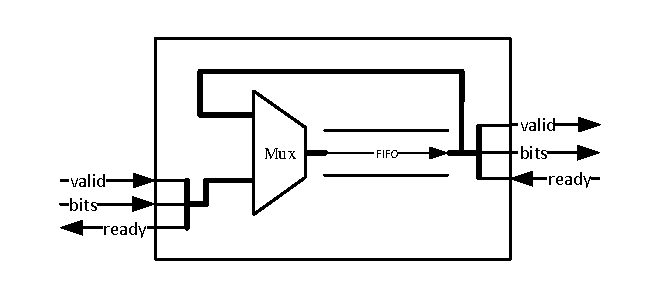
\includegraphics[scale=1.1]{../pdf/fifoshift.pdf}\\
    \caption{基于FIFO构造的移位寄存器}
\end{figure}
\begin{table}[h] %开始一个表格environment,表格的位置是h,here。  
    \centering
    \caption{基于FIFO构造的移位寄存器端口说明} %显示表格的标题  
    \begin{tabular}{l|l|c|l} %设置了每一列的宽度,强制转换。  
    \hline  
    \hline  
    端口 & 类型 & 位宽 & 功能 \\ %用&来分隔单元格的内容 \\表示进入下一行  
    \hline %画一个横线,下面的就都是一样了,这里一共有4行内容  
    valid 左 & Input & 1 & 来自生产者的握手信号 \\  
    \hline  
    bits 左 & Input & 1 & 来自生产者的数据 \\  
    \hline  
    ready 左 & Output & w\footnotemark[1] &输出至生产者的握手信号 \\  
    \hline  
    valid 右 & Output & 1 & 输出至消费者的握手信号 \\  
    \hline  
    bits 右 & Output & w & 输出至消费者的数据 \\  
    \hline  
    ready 右 & Input & 1 & 来自消费者的握手信号\\  
    \hline  
    control & Input & 1 & 来自外界的控制内嵌FIFO功能的信号\\  
    \hline  
    \hline  
    \end{tabular}  
\end{table}
\footnotetext[1]{w表示该信号位宽可配置,下文意义相同}
利用FIFO的先入先出特性,配合外部控制信号可以构造一个最大位宽为FIFO深度的移位寄存器。
首先,模块中的Mux将FIFO接口入模块输入信号连接,此时数据被写入FIFO中,当数据输入过程完成之后,Mux将模块内的FIFO输入与输出对接,
此时便形成了一个数据环路,FIFO输出的数据被输入给FIFO的输入,使数据一直保留在FIFO中。该模块工作工程可参考图\ref{shift_k}。
\begin{figure}[h]
    \centering
    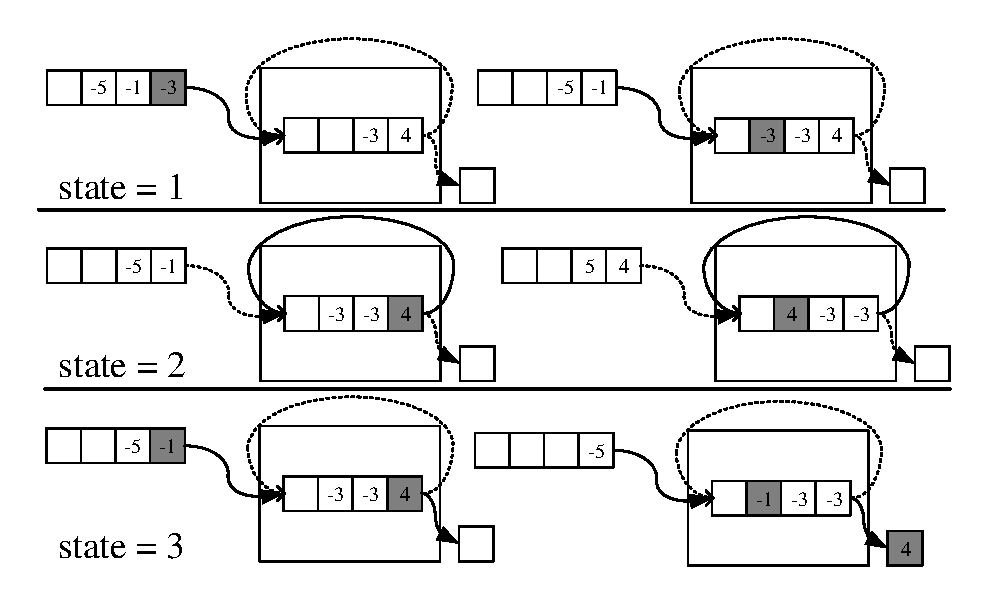
\includegraphics[scale=0.8]{../pdf/shift_k.pdf}\\
    \caption{基于FIFO的可变长移位寄存器工作示意图}
    \label{shift_k}
\end{figure}
实际使用时,FIFO深度被配置为256,位宽为16bit。第一阶段,FIFO输入通过Mux与模块的输入对接,接受来自外部的图像或者卷积核信息,第一阶段取数完成后进入第二阶段——计算,此时FIFO的输入与FIFO的输出对接,吐出的数据再次被存入FIFO中,以达到移位寄存器的功能。

需要说明的是,由于FIFO先入先出的特性,该移位构造,读数时每次只能读取最末端的数据,但相比与传统通过寄存器的构造,降低了资源占用率。

    \subsection{BRAM与DRAM选择}
    在Xilinx 7系FPGA中,片上RAM分为BRAM和DRAM两种,其中BRAM为板载RAM,是专门用于实现大容量RAM的部分,而DRAM是通过LUT构造的RAM。实际使用时,大容量RAM通常使用BRAM,但BRAM使用较为笨重,因为其是FPGA中的位置固定,会造成连线传输延时高的问题,同时BRAM时序比较严格,必须使用同步写入、同步读取的方式进行操作。而DRAM相对灵活,由于采用LUT构造,其能出现在FPGA绝大部分位置来最小化传输延时,同时DRAM可以进行异步读取操作,也可以在其后添加寄存器实现同步读取操作。本文所阐述的方案由于需要RAM具有异步读取操作,同时RAM容量小,数量多,因此采用DRAM。

\section{SRAM部分在FPGA中的优化}
\begin{figure}[h]
    \centering
    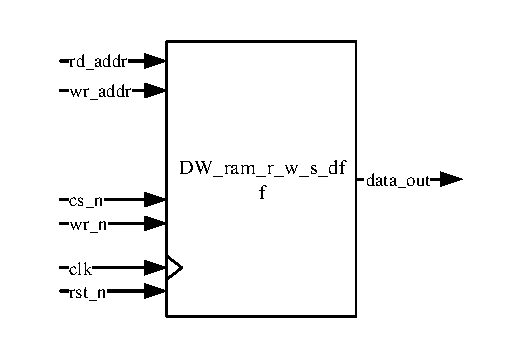
\includegraphics{../pdf/sram.pdf}\\
    \caption{使用Designware中的SRAM IP核接口图}
\end{figure}
\begin{table}[h] %开始一个表格environment,表格的位置是h,here。  
    \centering
    \caption{调用的Designware中的SRAM IP端口说明} %显示表格的标题  
    \begin{tabular}{l|l|c|l} %设置了每一列的宽度,强制转换。  
    \hline  
    \hline  
    端口 & 类型 & 位宽 & 功能 \\ %用&来分隔单元格的内容 \\表示进入下一行  
    \hline %画一个横线,下面的就都是一样了,这里一共有4行内容  
    clk & Input & 1 & 时钟信号 \\  
    \hline  
    rst\_n & Input & 1 & 复位信号 低有效 \\  
    \hline  
    cs\_n & Input & 1 & 片选信号 低有效 \\  
    \hline  
    wr\_n & Input & 1 & 写使能 低有效\\  
    \hline  
    rd\_addr & Input & $log_2[depth]$ & 读地址 \\  
    \hline  
    wr\_addr & Input & $log_2[depth]$ & 写地址 \\  
    \hline  
    data\_in & Input & w & 输入数据总线\\  
    \hline  
    data\_out & Output & w & 输出数据总线\\  
    \hline  
    \hline  
    \end{tabular}  
\end{table}  
Chisel3中构造存储器有两种方式,第一种通过VecInit构造ROM,FPGA实现时是通过线网。第二种通过MEM构造RAM,FPGA实现时是通过寄存器组。本文在设计过程中,首先通过MEM来构造片上RAM,但由于Chisel3 MEM自身的复杂度(其包含了Mask等附加功能),在实现一个6×7的PE阵列时,生成的代码量达到了16万行,通过Vivado综合一次需要90分钟,给调试工作带来了极大的不便利性,同时采用寄存器组的实现方式十分消耗资源。

由于ASIC中RAM通常需要特殊对待,本文在实际开发时,采用了Designware中的\emph{DW\_ram\_r\_w\_s\_dff}ip核。优化之后生成的代码量由16万下降至4万行,Vivado综合实现时间由90分钟下降至5分钟。同时Designware中提供了ip的仿真模型,可以通过Verilator仿真器进行准确的仿真。

% \section{基于Xilixn 7Series FPGA片上DSP的高性能乘法器}

\section{PE单元构造}
\begin{figure}[h]
    \centering
    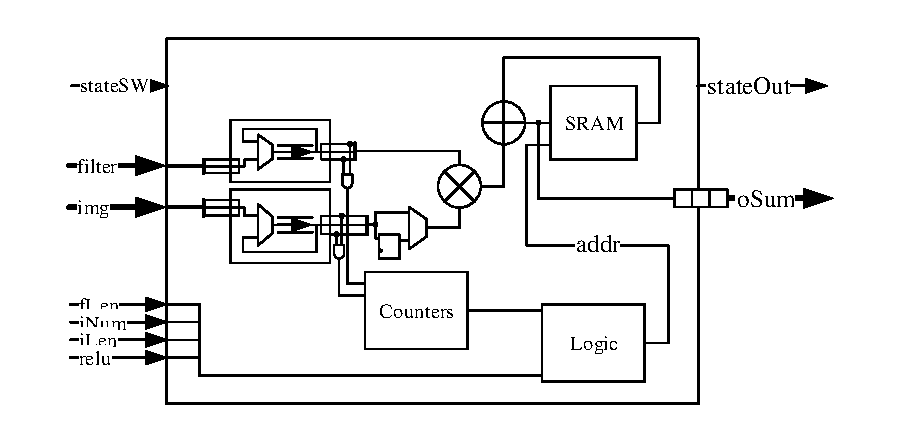
\includegraphics{../pdf/PE.pdf}\\
    \caption{PE结构图}
\end{figure}
\begin{figure}[h]
    \centering
    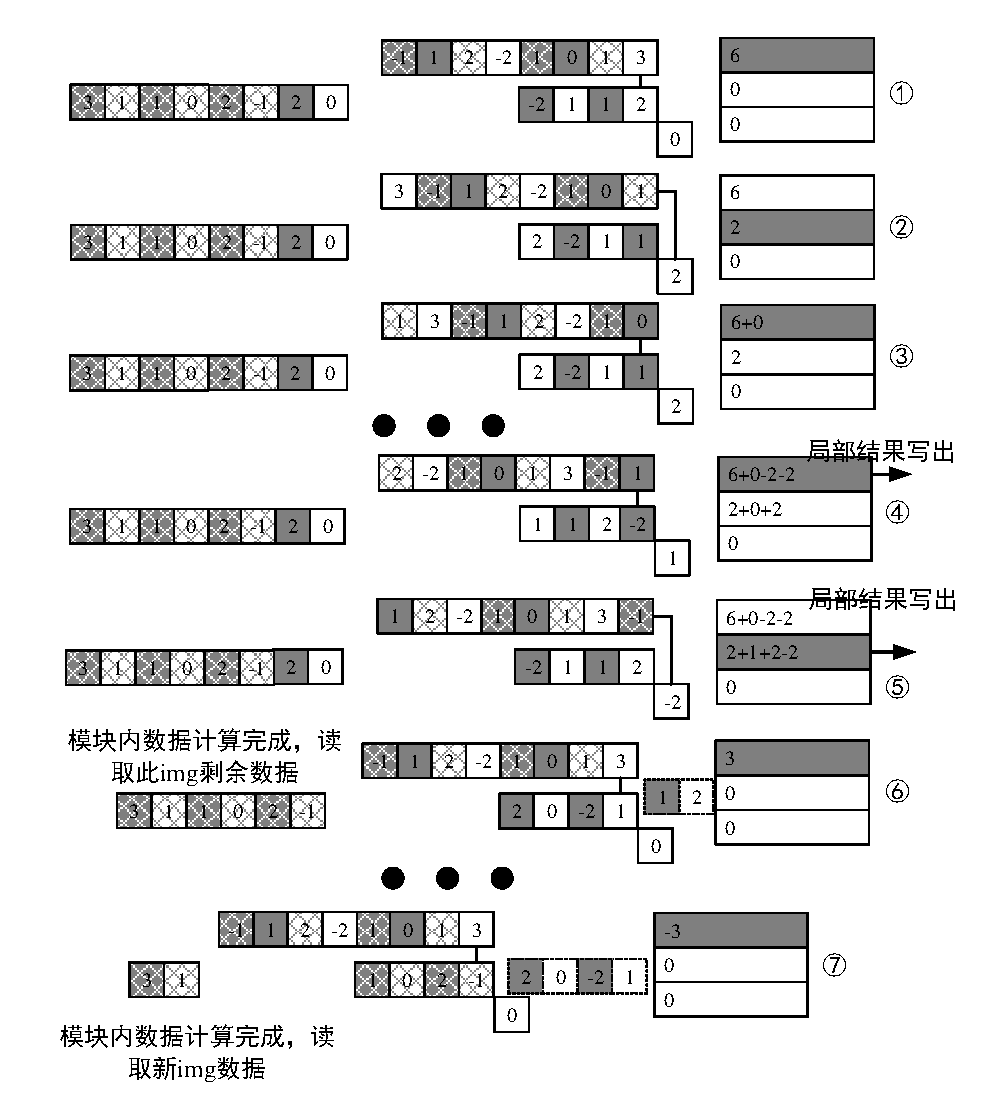
\includegraphics{../pdf/pe_cal.pdf}\\
    \caption{PE计算流程图}
\end{figure}
\begin{table}[h] %开始一个表格environment,表格的位置是h,here。  
    \centering
    \caption{PE单元端口说明} %显示表格的标题  
    \begin{tabular}{l|l|c|l} %设置了每一列的宽度,强制转换。  
    \hline  
    \hline  
    端口 & 类型 & 位宽 & 功能 \\ %用&来分隔单元格的内容 \\表示进入下一行  
    \hline %画一个横线,下面的就都是一样了,这里一共有4行内容  
    stateSW & Input & 2 & 状态切换信号 \\
    \hline  
    filter & Flipped-DecoupleIO & w & 输入filter解耦信号 \\
    \hline  
    img & Flipped-DecoupleIO & w & 输入filter解耦信号 \\
    \hline  
    fLen & Input & 8 & 单个filter长度 \\
    \hline  
    fNum & Input & 8 & 输出通道数 \\
    \hline  
    iLen & Input & 8 & 单个img长度 \\
    \hline  
    iNum & Input & 8 & 输入通道数 \\
    \hline  
    relu & Input & 1 & 进行Relu激活高有效 \\
    \hline  
    stateOut & Output & 2 & 输出当前状态 \\
    \hline  
    oSum & Output & w & 输出数据总线 \\
    \hline  
    \hline  
    \end{tabular}  
\end{table}  
利用本章第一节和第二节所述的两个模块,配合相应的控制单元可以十分完美的构造一个用于行静止思想卷积的PE(Process Engine)单元。


\section{用于数据分发的简易NoC设计}
\begin{figure}[h]
    \centering
    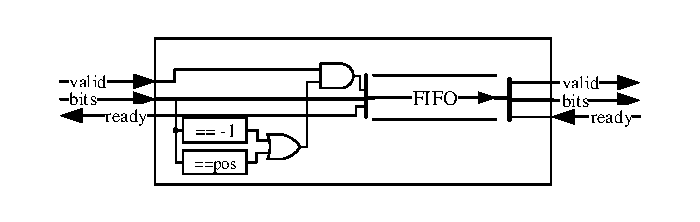
\includegraphics{../pdf/node.pdf}\\
    \caption{简易NoC中的一个节点构造}
\end{figure}
\begin{table}[h] %开始一个表格environment,表格的位置是h,here。  
    \centering
    \caption{简易NoC节点端口说明} %显示表格的标题  
    \begin{tabular}{l|l|c|l} %设置了每一列的宽度,强制转换。  
    \hline  
    \hline  
    端口 & 类型 & 位宽 & 功能 \\ %用&来分隔单元格的内容 \\表示进入下一行  
    \hline %画一个横线,下面的就都是一样了,这里一共有4行内容  
    valid 左 & Input & w & 来自生产者的握手信号 \\
    \hline  
    bits 左 & Input & w & 来自生产者的数据 \\
    \hline  
    ready 左 & Output & 8 & 输出给生产者的握手信号 \\
    \hline  
    valid 右 & Output & 8 & 输出给消费者的握手信号 \\
    \hline  
    bits 右 & Output & 8 & 输出给消费者的数据 \\
    \hline  
    ready 右 & Input & 8 & 来自消费者的握手信号 \\
    \hline  
    \hline  
    \end{tabular}  
\end{table}  
\begin{figure}[h]
    \centering
    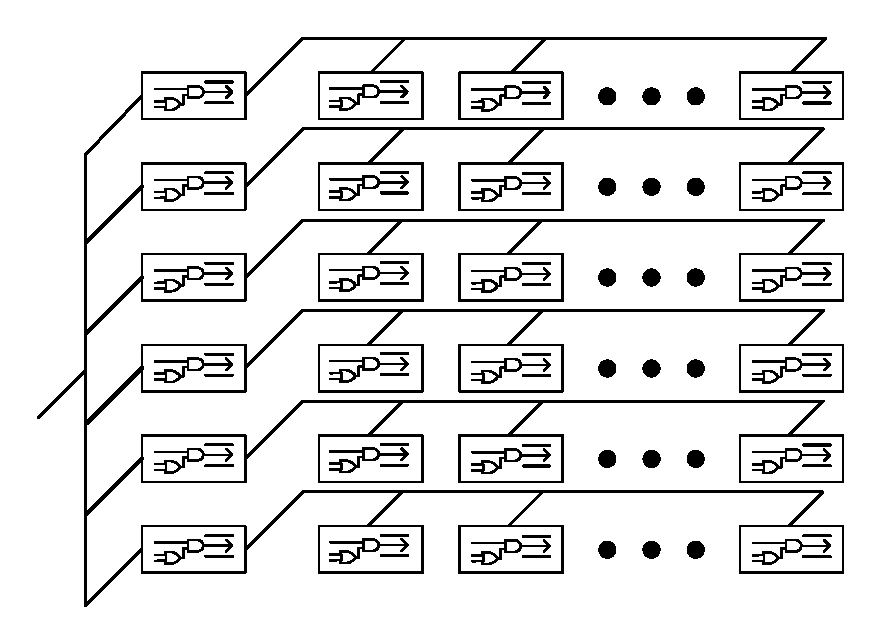
\includegraphics{../pdf/noc.pdf}\\
    \caption{简易NoC示意图}
\end{figure}
NoC(Network-on-Chip)及片上网络,是SoC的一种全新的通信方式,相比于传统总线式通信,基于NoC的系统能更好的适应全局异步局部同步的时钟机制。
但一个完整的NoC系统极其复杂,通信时的数据要经过打包、缓冲、同步等步骤,增加了延时的同时也增加了电路复杂度,不利于缩小电路面积。

实际使用时,本着轻量化的思想,本文所构造的NoC在空间中划分了一个二维节点矩阵,第一个列的节点用于行分发,其余列的节点用于列分发。

\section{PE阵列生成器}
\begin{figure}[h]
    \centering
    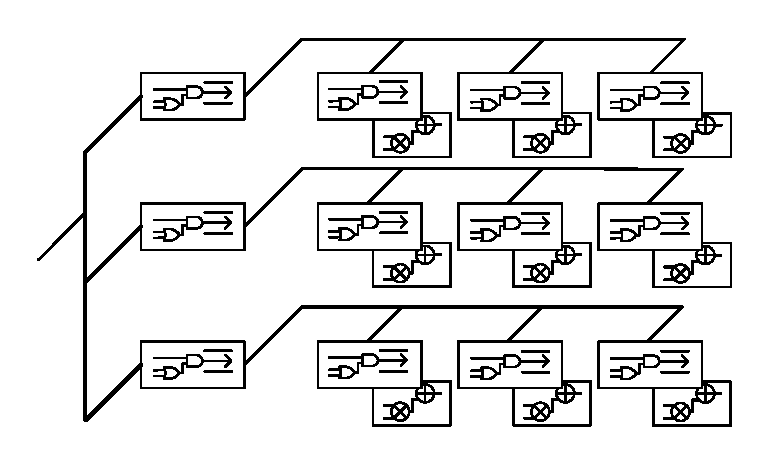
\includegraphics{../pdf/PEArray.pdf}\\
    \caption{一个3×3PE阵列示意图}
\end{figure}
Chisel3敏捷的一方面就体现在其可以利用Scala中的数据结构来组织硬件电路。在构造PE阵列的时候,本文采用了List。
    \subsection{顶层接口设计}
\begin{table}[h] %开始一个表格environment,表格的位置是h,here。  
    \centering
    \caption{PE阵列端口说明} %显示表格的标题  
    \begin{tabular}{l|l|c|l} %设置了每一列的宽度,强制转换。  
    \hline  
    \hline  
    端口 & 类型 & 位宽 & 功能 \\ %用&来分隔单元格的内容 \\表示进入下一行  
    \hline %画一个横线,下面的就都是一样了,这里一共有4行内容  
    stateSW & Input & 2 & 状态切换信号 \\
    \hline  
    config & Input & w & 传入PE单元计算需要的配置信息 \\
    \hline  
    dataIn & Flipped-DecoupleIO & w & 传入数据包括地址、类型、数据 \\
    \hline  
    oSum & DecoupleIO & w & 输出计算结果 \\
    \hline  
    done & Output & 1 & 计算完成标志高有效 \\
    \hline  
    \hline  
    \end{tabular}  
\end{table}  
    \subsection{计算流程}

\section{本章小结}
% \subsection{二级节标题}

% \subsubsection{三级节标题}

% \paragraph{四级节标题}

% \subparagraph{五级节标题}

% \section{脚注}

% Lorem ipsum dolor sit amet, consectetur adipiscing elit, sed do eiusmod tempor
% incididunt ut labore et dolore magna aliqua. Ut enim ad minim veniam, quis
% nostrud exercitation ullamco laboris nisi ut aliquip ex ea commodo consequat.
% Duis aute irure dolor in reprehenderit in voluptate velit esse cillum dolore eu
% fugiat nulla pariatur. Excepteur sint occaecat cupidatat non proident, sunt in
% culpa qui officia deserunt mollit anim id est laborum.
% \footnote{This is a long long long long long long long long long long long long
% long long long long long long long long long long footnote.}
